\documentclass[a4paper]{article}
\usepackage{geometry}
\usepackage{multicol}
\usepackage{setspace}
\usepackage{listings}
\usepackage{graphicx}
\usepackage{algorithm}
\usepackage{algpseudocode}
\usepackage{amsmath}
\usepackage{amssymb}
\usepackage{multicol}
\usepackage{float}
\DeclareGraphicsExtensions{.eps,.ps,.jpg,.bmp}
\usepackage{xcolor}
%\setlength{\parskip}{0.5\baselineskip}
\geometry{left=2.5cm,right=2.5cm,top=1.5cm,bottom=2.0cm} 
\title{\textbf{Algorithmn HW9}}
\author{5140379032 JIN YI FAN}
\date{}
\begin{document}
\maketitle
\begin{spacing}{1.3}
%\begin{multicols}{2}
\begin{multicols}{2}
\section*{Problem 7.5}
%\begin{multicols}{2}
\begin{figure}[H]
    \centering
    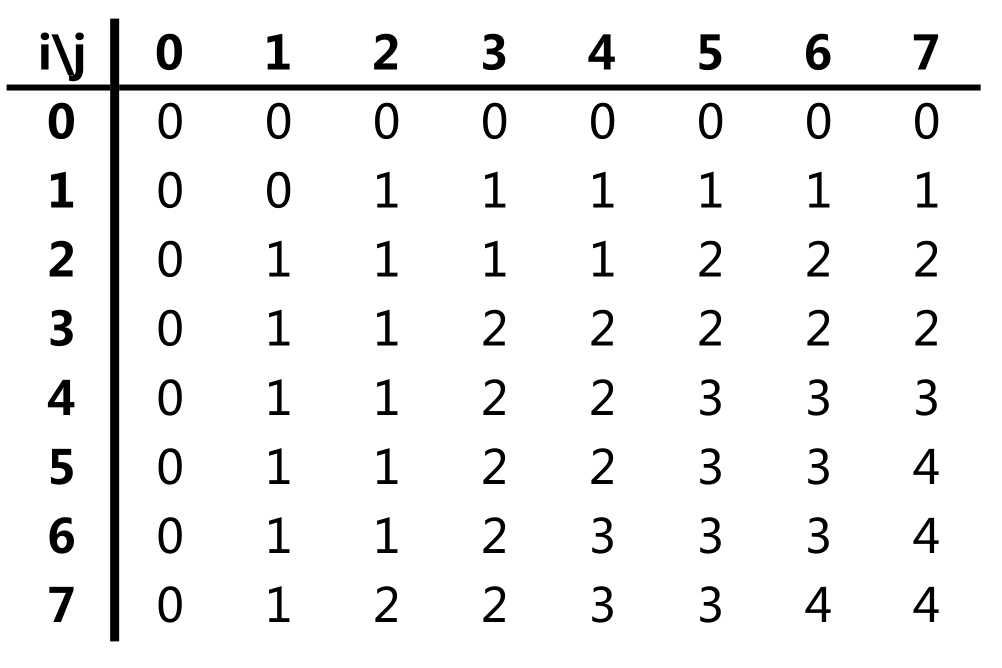
\includegraphics[width=4.5cm]{LCS.png}
\end{figure}
The figure on the left shows the result matrix of the DP.
\\So the length of longest common subsequence is $4$, and the longest common subsequence of $xzyzzyx$ and $zxyyzxz$ is $zyzz$.
%\end{multicols}

\section*{Problem 7.11}
\begin{figure}[H]
    \centering
    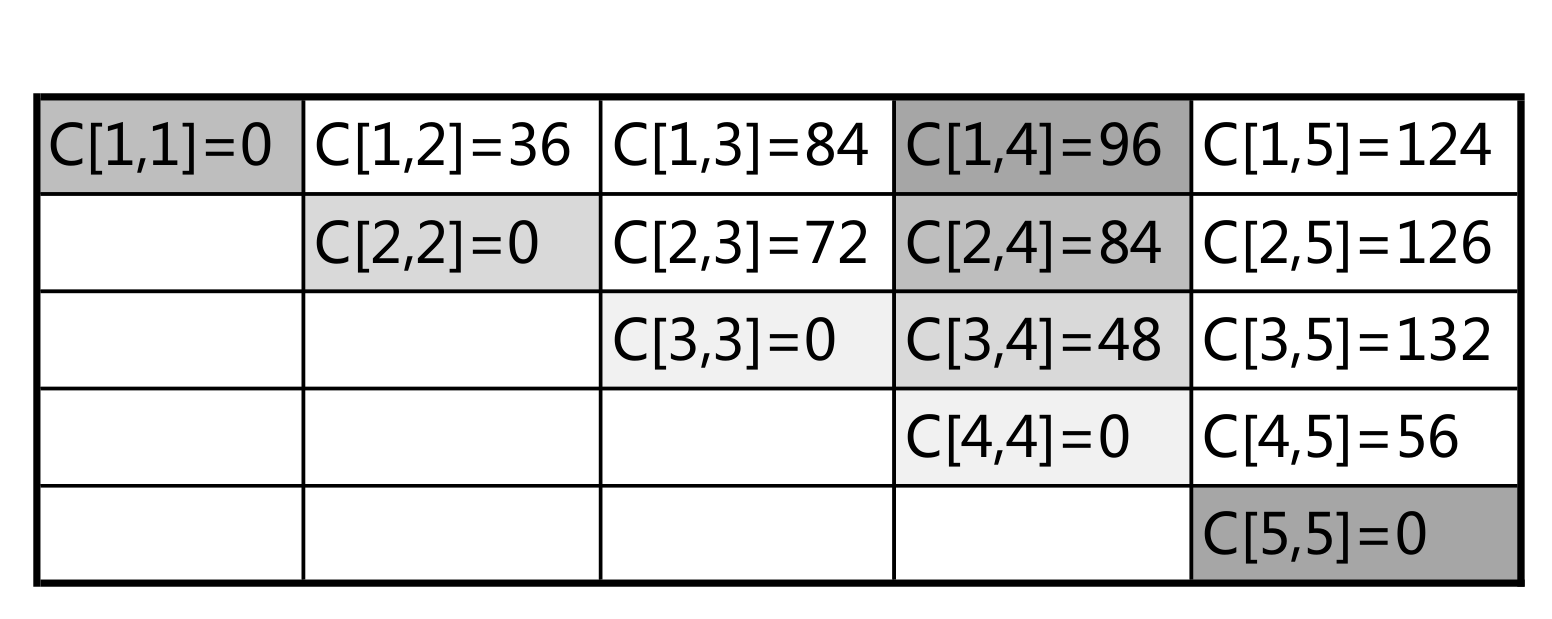
\includegraphics[width=6.5cm]{matrix.png}
\end{figure}
\textbf{(a).}According to the figure above, we can conclude that the minimum number of scalar multiplications needed is $C[1,5]=124$.
\\\textbf{(b).}To achieve optimal situation, the order should be $M_1\times (M_2\times (M_3\times M_4))\times M_5$
\end{multicols}

\section*{Problem 7.26}
\begin{multicols}{2}
The running time will be $\Theta(n\lfloor C/K\rfloor)$
\\Counterexample: Suppose $C=12$
\begin{table}[H]
\centering  
\begin{tabular}{lccc}
\hline
$s_i$  &1 &11 &10\\ \hline  
$v_i$ &1 &1 &1\\ \hline
\end{tabular}
\end{table}
when $K=6$, it will be $C=2$ and
\begin{table}[H]
\centering  
\begin{tabular}{lccc}
\hline
$\lfloor s_i/K\rfloor$  &0 &1 &1\\ \hline  
$v_i$ &1 &1 &1\\ \hline
\end{tabular}
\end{table} 
Obviously, some $s_i$ become $0$ and meaningless.
\end{multicols}

\section*{Problem 7.30}
\textbf{(a)}
\begin{algorithmic}[1]
\Require total value $y$ and a sequence of coin value $\{ v_1=1,v_2\ldots v_n\}$
\Ensure the pay plan $\{x_1,x_2\ldots x_n\}$
\State $dp[j\gets 0$ to $y ]\gets (j==0?\ 0:-1)$
\For{$i\gets 1$ to $n$}
\For{$j\gets v_i$ to $y$}
\State $dp[j]=min\{dp[j],dp[j-v_i]+1\}$\Comment{find the minimum volume}
\State $take[j]=i$ if $dp[j]==dp[j-v_i]+1$\Comment{store the adding coin}
\EndFor
\EndFor
\State $j\gets y$
\While{$dp[j]!=-1$}\Comment{recover the plan}
\State $x_{take[j]}\gets x_{take[j]}+1$
\State $j\gets j-v_{take[j]}$
\EndWhile
\end{algorithmic}
\textbf{(b)} Time complexity is $O(y\cdot n)$, space complexity is $O(y)$
\\\textbf{(c)}
Problem 7.27, the complete knapsack problem is to \textbf{maximize} $value$ with $volume$ constraint, 
\\while this problem is to \textbf{minimize} $volume$(which is $1$ for each) with $value$ constraint.

\section*{Problem 7.34}
\begin{algorithmic}[1]
\Require a DAG $G=(V,E)$, start point $s$ and end point $t$
\Ensure a longest path $P=\{s\ldots t\}$
\State \Call{topoSort}{V}
\State $dp[s]\gets 0$\Comment{$dp[i]$ means the longest path end with $i$}
\For{each $v\in V$ s.t. $s<v\leq t$}
\State $dp[v]\gets max_{(u,v)\in E}\{dp[u]+w(u,v)\}$\Comment{check every edge connected}
\State $pred[v]\gets u$ s.t. $w(u,v)$ is maximum \Comment{store the predecessor of each vertex}
\EndFor
\State \textbf{return} $dp[t]$
\end{algorithmic}

\section*{SubsetSum}
\begin{algorithmic}[1]
\Require a list of $n$ positive integers $a_1,a_2\ldots a_n$, a positive integer $t$.
\Ensure whether there is some subset of $a_i$s add up to $t$
\For{$i\gets 0$ to $n$}
\State $T[i,0]\gets 0$\Comment{$T[i,s]$ is the boolean value of 'does a subset $\{a_1\ldots a_i\}$ add up to $s$?'}
\EndFor
\For{$i\gets 1$ to $n$}
\For{$s\gets 1$ to $t$}
\State $T[i,s]\gets T[i-1,s]\ |\ T[i-1,s-a_i]$
\EndFor
\EndFor
\State \textbf{return} $T(n,t)$
\end{algorithmic}

\section*{PickCards}
\textbf{(a)} Consider the sequence $2,100,1,1$, using $greedy$ strategy, the first player will take the front $2$, and the second player will take $100$ and win the game. 
\\\textbf{(b)}
\begin{algorithmic}[1]
\State $dp[i][0]\gets 0$ for each $i\in range(0,n+1)$
\State $dp[0][j]\gets 0$ for each $j\in range(0,n+1)$
\State $dp[i][i]\gets s_i$ for each $i\in range(1,n+1)$
\For{$i\gets 1$ to $n$}
\For{$j\gets i+1$ to $n$}
\State $first\gets min(dp[i+2][j],dp[i+1][j-1])+s_i$\Comment{p1: take first, p2:min(take first, take last)}
\State $last\gets min(dp[i][j-2],dp[i+1][j-1])+s_j$\Comment{p1: take last, p2:min(take last, take first)}
\State $pred[i][j]\gets first>last?\ s_i:s_j$
\State $dp[i][j]\gets max(first,last)$
\EndFor
\EndFor\Comment{Then player can refer to the $pred$ matrix to make the optimal decision for each step}

\end{algorithmic}
%\end{multicols}
\end{spacing}
\end{document}

